\newpage
\section[Визуализация баллистического движения]{Визуализация баллистического движения}

Требуется визуализировать движение тела, брошенного под углом к горизонту с учетем сопротивления ветра.
Для упрощения модели сопротивление ветра задается постоянной силой, направленной против направления проекции начальной скорости тела на оcь Ox.

Имеем уравнения движения тела в проекциях на оси:
\begin{equation*}
    \begin{aligned}
        &y(t) = y_{0} + v_{0y}t+\frac{a_{y}t^{2}}{2}; \\
        &x(t) = x_{0} + v_{0x}t+\frac{a_{x}t^{2}}{2}
    \end{aligned}
\end{equation*}

Разложим начальную скорость на проекции
\begin{equation*}
    \begin{aligned}
        &v_{0y} = v_{0} \cdot Sin(\alpha); \\
        &v_{0x} = v_{0} \cdot Cos(\alpha)
    \end{aligned}
\end{equation*}

По второму закону Ньютона:
\begin{equation*}
    m\vec{a} = m\vec{g} + \vec{F}_{\text{сопр}} \\
\end{equation*}

В проекциях на оси:
\begin{equation*}
    \begin{aligned}
        &Oy: \; ma_{y} = -mg; \;\; 
        a_{y} = -g; \\
        &Ox: \; ma_{x} = -F_{\text{сопр}} \;\;
        a_{x} = -\frac{F_{\text{сопр}}}{m} 
    \end{aligned}
\end{equation*}

Конечные уравнения движения тела:
\begin{equation*}
    \begin{aligned}
        &y(t) = y_{0} + v_{0}t \cdot Sin(\alpha) - \frac{gt^{2}}{2};\\
        &x(t) = x_{0} + v_{0}t \cdot Cos(\alpha) - \frac{F_{\text{сопр}}t^{2}}{2m}
    \end{aligned}
\end{equation*}

Конечная система дифференциальных уравнений:
\begin{equation*}
    \left\{
        \begin{aligned}
            &x(0) = 0 \\
            &x'(0) = v_{0} \cdot Cos(\alpha) \\
            &x''(t) = \frac{-F_{\text{сопр}}}{m}
        \end{aligned}
    \right.; \;\;\;\;\;\;\;\;\;
    \left\{
        \begin{aligned}
            &y(0) = 0 \\
            &y'(0) = v_{0} \cdot Sin(\alpha) \\
            &y''(t) = -g
        \end{aligned}
    \right. \end{equation*}

\newpage
Моделируем полет тела в Wolfram Mathematicа. 
Ипользуем инструменты 
\textbf{NDSolve}, 
\textbf{Evaluate},
\textbf{ParametricPlot}\\

\textit{Листинг программы Matematica:}
\begin{figure}[ht]
    \begin{lstlisting}
(* Исходные параметры *)
v = 28.4;
angle = Pi/3;
g = 9.8;
ResistForce = 4;
Mass = 2;

(* Получение численного решения систем дифференциальных уравнений *)
ndsY = NDSolve[
    {y''[t] == -g, y'[0] == v * Sin[angle], y[0] == 0}, 
    y, 
    {t, 0, 10}
];
   
ndsX = NDSolve[
    {x''[t] == -ResistForce / Mass, x'[0] == v*Cos[angle], x[0] == 0}, 
    x, 
    {t, 0, 10}
];

(* Построение графика *)
ParametricPlot[
    {Evaluate[{x[t], y[t]} /. Flatten@{ndsX, ndsY}]}, 
    {t, 0, 5},
    AxesLabel -> {x, y}
] 
    \end{lstlisting} 
\end{figure}\\
\textit{Полученный график:}
\begin{figure}[ht]
\centering
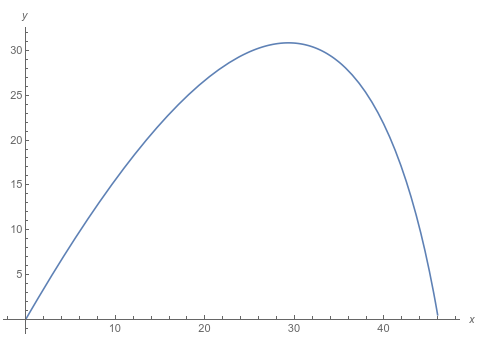
\includegraphics[width=0.4\linewidth]{5-ballistic.png}
\end{figure}
